\documentclass[aspectratio=169,11pt]{beamer}

% Theme and colors
\usetheme{Madrid}
\usecolortheme{whale}
\setbeamertemplate{navigation symbols}{}
\setbeamertemplate{footline}[frame number]

% Packages
\usepackage[utf8]{inputenc}
\usepackage[T1]{fontenc}
\usepackage{graphicx}
\usepackage{booktabs}
\usepackage{amsmath}
\usepackage{hyperref}
\usepackage{tikz}
\usetikzlibrary{shapes,arrows,positioning,calc,fit,backgrounds,decorations.pathmorphing}
\usepackage{siunitx}

% Bibliography
\usepackage[backend=biber,style=ieee,sorting=none]{biblatex}
\addbibresource{references.bib}

% Custom colors for questions
\definecolor{questionbg}{RGB}{255,248,220}
\definecolor{questionborder}{RGB}{255,193,7}

% Title information
\title[EECE5155 -- Module 4 Part 2]{IoT Communication Protocols}
\subtitle{Module 4 Part 2: Standards, Specifications, and Selection}
\author{Eduardo Baena}
\date{Spring 2026}
\institute{Northeastern University\\Department of Electrical and Computer Engineering\\
\texttt{e.baena@northeastern.edu}}

\begin{document}

% Title slide
\begin{frame}
    \titlepage
    \vspace{-1cm}
    \begin{center}
        \textbf{EECE5155: Wireless Sensor Networks and the Internet of Things}
    \end{center}
\end{frame}

% Learning Objectives
\begin{frame}{Learning Objectives}
    \textbf{By the end of this module, you should be able to:}
    
    \vspace{0.5cm}
    \begin{enumerate}
        \item \textbf{Compare} IoT protocols using verified technical specifications
        \item \textbf{Calculate} link budgets from datasheet parameters
        \item \textbf{Select} the appropriate protocol for your application requirements
        \item \textbf{Justify} your protocol choice with quantitative analysis
        \item \textbf{Document} communication requirements in your PES
    \end{enumerate}
    
    \vspace{0.3cm}
    \begin{alertblock}{Engineering Standard}
        Every specification in this module comes from \textbf{official standards documents} or \textbf{manufacturer datasheets}. You must cite similarly in your PES.
    \end{alertblock}
\end{frame}

% Outline
\begin{frame}{Outline}
    \tableofcontents
\end{frame}

%==============================================================================
\section{Link Budget Fundamentals}
%==============================================================================

\begin{frame}{Why Link Budget Matters}
    \textbf{The link budget determines if your wireless system will work.}
    
    \vspace{0.3cm}
    \begin{center}
    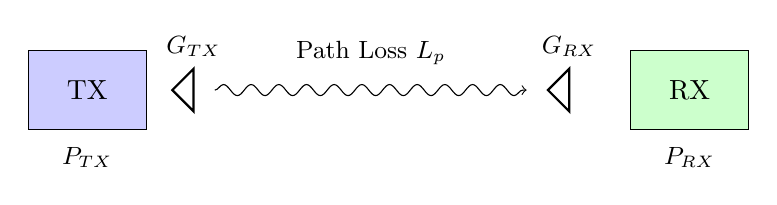
\begin{tikzpicture}[scale=0.9]
        % TX
        \node[draw, fill=blue!20, minimum width=1.5cm, minimum height=1cm] (tx) at (0,0) {TX};
        \node[below=0.1cm of tx, font=\small] {$P_{TX}$};
        
        % Antenna TX
        \draw[thick] (1.2,0) -- (1.5,0.3) -- (1.5,-0.3) -- cycle;
        \node[above=0.3cm, font=\small] at (1.5,0) {$G_{TX}$};
        
        % Path
        \draw[decorate, decoration={snake, amplitude=2pt, segment length=10pt}, ->] (1.8,0) -- (6.2,0);
        \node[above=0.2cm, font=\small] at (4,0) {Path Loss $L_p$};
        
        % Antenna RX
        \draw[thick] (6.5,0) -- (6.8,0.3) -- (6.8,-0.3) -- cycle;
        \node[above=0.3cm, font=\small] at (6.8,0) {$G_{RX}$};
        
        % RX
        \node[draw, fill=green!20, minimum width=1.5cm, minimum height=1cm] (rx) at (8.5,0) {RX};
        \node[below=0.1cm of rx, font=\small] {$P_{RX}$};
    \end{tikzpicture}
    \end{center}
    
    \vspace{0.3cm}
    \begin{block}{Link Budget Equation}
        \[
        P_{RX} = P_{TX} + G_{TX} - L_p + G_{RX} - L_{misc} \quad \text{[all in dB]}
        \]
    \end{block}
    
    \textbf{Success criterion:} $P_{RX} > S_{RX}$ (receiver sensitivity)
\end{frame}

\begin{frame}{Power Units: Watts vs. dBm vs. dBW}
    \textbf{Linear vs. Logarithmic Units}
    
    \vspace{0.3cm}
    \begin{columns}[T]
        \begin{column}{0.48\textwidth}
            \textbf{Linear (Watts):}
            \begin{itemize}
                \item Used for energy calculations
                \item $P = V \times I$ [W]
                \item $E = P \times t$ [J]
                \item Multiplication for gains/losses
            \end{itemize}
            
            \vspace{0.3cm}
            \textbf{Logarithmic (dB):}
            \begin{itemize}
                \item Used for link budgets
                \item Addition for gains/losses
                \item Easier to handle large ranges
            \end{itemize}
        \end{column}
        \begin{column}{0.48\textwidth}
            \textbf{Conversion Formulas:}
            \begin{align*}
                P_{dBm} &= 10 \log_{10}\left(\frac{P_{mW}}{1 \text{ mW}}\right) \\[0.3cm]
                P_{dBW} &= 10 \log_{10}\left(\frac{P_{W}}{1 \text{ W}}\right) \\[0.3cm]
                P_{dBm} &= P_{dBW} + 30
            \end{align*}
        \end{column}
    \end{columns}
    
    \vspace{0.3cm}
    \begin{alertblock}{Common Mistake}
        Never add powers in Watts directly in link budgets. Convert to dB first!
    \end{alertblock}
\end{frame}

\begin{frame}{Power Reference Table}
    \begin{table}
        \centering
        \begin{tabular}{@{}lccc@{}}
            \toprule
            \textbf{Description} & \textbf{Watts} & \textbf{dBm} & \textbf{dBW} \\
            \midrule
            WiFi router (typical) & 100 mW & +20 dBm & $-$10 dBW \\
            BLE TX (0 dBm) & 1 mW & 0 dBm & $-$30 dBW \\
            LoRa TX (+14 dBm) & 25 mW & +14 dBm & $-$16 dBW \\
            NB-IoT TX (+23 dBm) & 200 mW & +23 dBm & $-$7 dBW \\
            \midrule
            BLE sensitivity & 50 pW & $-$93 dBm & $-$123 dBW \\
            LoRa sensitivity (SF12) & 2 fW & $-$137 dBm & $-$167 dBW \\
            Thermal noise floor & 4 fW & $-$174 dBm/Hz & -- \\
            \bottomrule
        \end{tabular}
    \end{table}
    
    \vspace{0.3cm}
    \textbf{Key insight:} IoT receivers detect signals $10^{14}$ times weaker than transmitted!
    
    \vspace{0.2cm}
    \begin{block}{Rule of Thumb}
        Every 3 dB = 2$\times$ power. Every 10 dB = 10$\times$ power.
    \end{block}
\end{frame}

%------------------------------------------------------------------------------
% QUESTION: dB Conversion
%------------------------------------------------------------------------------
\begin{frame}{Think First}
    \begin{center}
    \fcolorbox{questionborder}{questionbg}{
    \begin{minipage}{0.85\textwidth}
        \vspace{0.3cm}
        \centering
        \Large\textbf{Question: Unit Conversion}
        
        \vspace{0.3cm}
        \normalsize
        A LoRa transceiver transmits at 100 mW.
        
        \vspace{0.3cm}
        \textbf{What is the TX power in dBm?}
        
        \vspace{0.3cm}
        \begin{enumerate}[A)]
            \item +10 dBm
            \item +17 dBm
            \item +20 dBm
            \item +23 dBm
        \end{enumerate}
        
        \vspace{0.3cm}
        Hint: $P_{dBm} = 10 \log_{10}(P_{mW})$
        \vspace{0.3cm}
    \end{minipage}
    }
    \end{center}
\end{frame}

\begin{frame}{Answer: Unit Conversion}
    \textbf{C) +20 dBm}
    
    \vspace{0.5cm}
    \textbf{Calculation:}
    \begin{align*}
        P_{dBm} &= 10 \log_{10}\left(\frac{100 \text{ mW}}{1 \text{ mW}}\right) \\[0.3cm]
        P_{dBm} &= 10 \log_{10}(100) \\[0.3cm]
        P_{dBm} &= 10 \times 2 = +20 \text{ dBm}
    \end{align*}
    
    \vspace{0.3cm}
    \textbf{Quick reference:}
    \begin{itemize}
        \item 1 mW = 0 dBm
        \item 10 mW = +10 dBm
        \item 100 mW = +20 dBm
        \item 1 W = +30 dBm
    \end{itemize}
\end{frame}

\begin{frame}{Path Loss Models}
    \textbf{How much signal is lost traveling through space?}
    
    \vspace{0.3cm}
    \textbf{Free Space Path Loss (FSPL):}
    \[
    L_{FSPL} = 20\log_{10}(d) + 20\log_{10}(f) - 147.55 \quad \text{[dB]}
    \]
    where $d$ = distance [m], $f$ = frequency [Hz]
    
    \vspace{0.3cm}
    \textbf{Log-Distance Path Loss (more realistic):}
    \[
    L_p = L_0 + 10n\log_{10}\left(\frac{d}{d_0}\right) \quad \text{[dB]}
    \]
    
    \begin{table}
        \centering
        \footnotesize
        \begin{tabular}{@{}lcc@{}}
            \toprule
            \textbf{Environment} & \textbf{Path Loss Exponent $n$} & \textbf{$L_0$ at 1m (2.4 GHz)} \\
            \midrule
            Free space & 2.0 & 40 dB \\
            Urban area & 2.7--3.5 & 40 dB \\
            Indoor (LOS) & 1.6--1.8 & 40 dB \\
            Indoor (NLOS) & 4--6 & 40 dB \\
            \bottomrule
        \end{tabular}
    \end{table}
    
    \textbf{Source:} Rappaport, \textit{Wireless Communications}, 2nd Ed.
\end{frame}

\begin{frame}{Receiver Sensitivity}
    \textbf{Minimum signal power the receiver can detect reliably.}
    
    \vspace{0.3cm}
    \begin{columns}[T]
        \begin{column}{0.48\textwidth}
            \textbf{Factors affecting sensitivity:}
            \begin{itemize}
                \item Noise figure (NF)
                \item Bandwidth (BW)
                \item Required SNR
                \item Modulation scheme
            \end{itemize}
            
            \vspace{0.2cm}
            \textbf{Sensitivity formula:}
            \[
            S = -174 + 10\log_{10}(BW) + NF + SNR_{req}
            \]
            \small{[dBm]}
        \end{column}
        \begin{column}{0.48\textwidth}
            \textbf{Typical sensitivities:}
            \begin{table}
                \centering
                \footnotesize
                \begin{tabular}{@{}lc@{}}
                    \toprule
                    \textbf{Protocol} & \textbf{Sensitivity} \\
                    \midrule
                    WiFi (54 Mbps) & $-$68 dBm \\
                    WiFi (6 Mbps) & $-$82 dBm \\
                    BLE (1 Mbps) & $-$93 dBm \\
                    Zigbee & $-$100 dBm \\
                    LoRa SF7 & $-$123 dBm \\
                    LoRa SF12 & $-$137 dBm \\
                    NB-IoT & $-$141 dBm \\
                    \bottomrule
                \end{tabular}
            \end{table}
        \end{column}
    \end{columns}
    
    \vspace{0.2cm}
    \begin{block}{Key Insight}
        Lower data rate $\rightarrow$ narrower bandwidth $\rightarrow$ better sensitivity $\rightarrow$ longer range
    \end{block}
\end{frame}

\begin{frame}{Link Margin: The Safety Factor}
    \textbf{Link Margin = Received Power $-$ Sensitivity}
    
    \vspace{0.3cm}
    \[
    M = P_{RX} - S_{RX} = (P_{TX} + G_{TX} - L_p + G_{RX}) - S_{RX} \quad \text{[dB]}
    \]
    
    \vspace{0.3cm}
    \begin{table}
        \centering
        \begin{tabular}{@{}lll@{}}
            \toprule
            \textbf{Margin} & \textbf{Reliability} & \textbf{Recommendation} \\
            \midrule
            $<$ 0 dB & Link fails & Redesign required \\
            0--5 dB & Unreliable & Not recommended \\
            5--10 dB & Marginal & Indoor/static only \\
            10--20 dB & Good & Typical design target \\
            $>$ 20 dB & Excellent & Mobile/harsh environments \\
            \bottomrule
        \end{tabular}
    \end{table}
    
    \vspace{0.2cm}
    \textbf{Why margin matters:}
    \begin{itemize}
        \item Fading (multipath, shadowing): 10--20 dB variation
        \item Temperature drift: 2--5 dB
        \item Antenna misalignment: 3--6 dB
        \item Component aging: 1--3 dB
    \end{itemize}
\end{frame}

%------------------------------------------------------------------------------
% QUESTION: Link Budget Calculation
%------------------------------------------------------------------------------
\begin{frame}{Think First}
    \begin{center}
    \fcolorbox{questionborder}{questionbg}{
    \begin{minipage}{0.85\textwidth}
        \vspace{0.3cm}
        \centering
        \Large\textbf{Question: Complete Link Budget}
        
        \vspace{0.3cm}
        \normalsize
        Calculate the link margin for a BLE connection:
        \begin{itemize}
            \item TX power: 0 dBm
            \item TX antenna gain: 0 dBi
            \item Distance: 30 m indoor (NLOS, $n$ = 4)
            \item $L_0$ = 40 dB at 1 m
            \item RX antenna gain: 0 dBi
            \item RX sensitivity: $-$93 dBm
        \end{itemize}
        
        \vspace{0.3cm}
        \textbf{Will this link work reliably?}
        \vspace{0.3cm}
    \end{minipage}
    }
    \end{center}
\end{frame}

\begin{frame}{Answer: Complete Link Budget}
    \textbf{Margin = $-$6 dB -- Link will NOT work reliably}
    
    \vspace{0.3cm}
    \textbf{Step 1: Calculate path loss}
    \begin{align*}
        L_p &= L_0 + 10n\log_{10}\left(\frac{d}{d_0}\right) \\
        L_p &= 40 + 10 \times 4 \times \log_{10}(30) \\
        L_p &= 40 + 40 \times 1.477 = 40 + 59 = 99 \text{ dB}
    \end{align*}
    
    \textbf{Step 2: Calculate received power}
    \begin{align*}
        P_{RX} &= P_{TX} + G_{TX} - L_p + G_{RX} \\
        P_{RX} &= 0 + 0 - 99 + 0 = -99 \text{ dBm}
    \end{align*}
    
    \textbf{Step 3: Calculate margin}
    \[
    M = P_{RX} - S_{RX} = -99 - (-93) = -6 \text{ dB} \quad \text{\textcolor{red}{FAIL}}
    \]
    
    \textbf{Solutions:} Increase TX power (+6 dBm), use directional antenna, reduce distance, or use LE Coded PHY ($-$103 dBm sensitivity).
\end{frame}

%==============================================================================
\section{IoT Protocol Landscape}
%==============================================================================

\begin{frame}{The Protocol Selection Problem}
    \begin{center}
    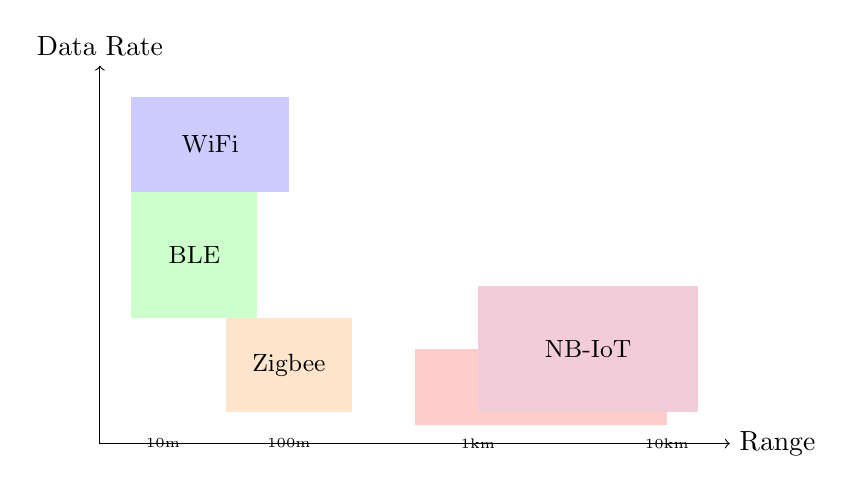
\begin{tikzpicture}[scale=0.8]
        % Axes
        \draw[->] (0,0) -- (10,0) node[right] {Range};
        \draw[->] (0,0) -- (0,6) node[above] {Data Rate};
        
        % Regions
        \fill[blue!20] (0.5,4) rectangle (3,5.5);
        \node[font=\small] at (1.75,4.75) {WiFi};
        
        \fill[green!20] (0.5,2) rectangle (2.5,4);
        \node[font=\small] at (1.5,3) {BLE};
        
        \fill[orange!20] (2,0.5) rectangle (4,2);
        \node[font=\small] at (3,1.25) {Zigbee};
        
        \fill[red!20] (5,0.3) rectangle (9,1.5);
        \node[font=\small] at (7,0.9) {LoRa};
        
        \fill[purple!20] (6,0.5) rectangle (9.5,2.5);
        \node[font=\small] at (7.75,1.5) {NB-IoT};
        
        % Labels
        \node[font=\tiny] at (1,0) {10m};
        \node[font=\tiny] at (3,0) {100m};
        \node[font=\tiny] at (6,0) {1km};
        \node[font=\tiny] at (9,0) {10km};
    \end{tikzpicture}
    \end{center}
    
    \vspace{0.2cm}
    \textbf{Your PES must answer:}
    \begin{itemize}
        \item What range do I need? (measured or calculated)
        \item What data rate do I need? (derived from sampling + packet size)
        \item What power budget do I have? (from Module 4 Part 1)
        \item What is my cost target? (infrastructure + per-node)
    \end{itemize}
\end{frame}

%------------------------------------------------------------------------------
% QUESTION 1
%------------------------------------------------------------------------------
\begin{frame}{Think First}
    \begin{center}
    \fcolorbox{questionborder}{questionbg}{
    \begin{minipage}{0.85\textwidth}
        \vspace{0.3cm}
        \centering
        \Large\textbf{Question 1}
        
        \vspace{0.3cm}
        \normalsize
        You need to deploy 100 temperature sensors in a warehouse (200m $\times$ 100m).\\
        Each sensor sends 20 bytes every 5 minutes.\\
        Battery life requirement: 2 years on 2$\times$AA batteries.
        
        \vspace{0.3cm}
        \textbf{Which protocol would you choose and why?}
        
        \vspace{0.3cm}
        \begin{enumerate}[A)]
            \item WiFi (802.11n)
            \item Bluetooth Low Energy 5.0
            \item Zigbee 3.0
            \item LoRaWAN
        \end{enumerate}
        \vspace{0.3cm}
    \end{minipage}
    }
    \end{center}
\end{frame}

\begin{frame}{Answer: Protocol Selection Analysis}
    \textbf{D) LoRaWAN or C) Zigbee -- depending on infrastructure}
    
    \vspace{0.2cm}
    \begin{table}
        \centering
        \footnotesize
        \begin{tabular}{@{}lcccc@{}}
            \toprule
            \textbf{Criterion} & \textbf{WiFi} & \textbf{BLE} & \textbf{Zigbee} & \textbf{LoRa} \\
            \midrule
            Range (indoor) & 50m & 30m & 100m & 500m+ \\
            Covers 200m? & No & No & Mesh & Yes \\
            TX current & 200 mA & 8 mA & 20 mA & 120 mA \\
            Sleep current & 50 $\mu$A & 1 $\mu$A & 1 $\mu$A & 0.2 $\mu$A \\
            2-year battery? & No & Yes & Yes & Yes \\
            Infrastructure & AP & Gateway & Coordinator & Gateway \\
            \bottomrule
        \end{tabular}
    \end{table}
    
    \vspace{0.2cm}
    \textbf{Decision:}
    \begin{itemize}
        \item \textbf{LoRaWAN:} Single gateway covers entire warehouse, lowest power
        \item \textbf{Zigbee:} Mesh extends range, but needs more nodes as routers
        \item WiFi/BLE: Insufficient range, WiFi too power-hungry
    \end{itemize}
\end{frame}

%==============================================================================
\section{LoRaWAN: Long Range, Low Power}
%==============================================================================

\begin{frame}{LoRaWAN Overview}
    \textbf{Standard:} LoRa Alliance TS001-1.0.4 (2022)
    
    \vspace{0.3cm}
    \begin{columns}[T]
        \begin{column}{0.48\textwidth}
            \textbf{Key Specifications:}
            \begin{itemize}
                \item Frequency: 868 MHz (EU), 915 MHz (US)
                \item Bandwidth: 125/250/500 kHz
                \item Data rate: 0.3--50 kbps
                \item Range: 2--15 km (rural), 1--5 km (urban)
                \item Sensitivity: up to $-$148 dBm
                \item TX power: up to +20 dBm
            \end{itemize}
        \end{column}
        \begin{column}{0.48\textwidth}
            \textbf{Power (SX1276 datasheet):}
            \begin{itemize}
                \item TX @ +14 dBm: 100 mA
                \item TX @ +20 dBm: 120 mA
                \item RX: 10.8 mA
                \item Sleep: 0.2 $\mu$A
                \item Startup: 1.5 ms
            \end{itemize}
            
            \vspace{0.2cm}
            \textbf{Source:} Semtech SX1276 DS, Rev. 7
        \end{column}
    \end{columns}
    
    \vspace{0.3cm}
    \begin{block}{Use Case}
        Long-range, low data rate, battery-powered sensors. Smart agriculture, asset tracking, utilities.
    \end{block}
\end{frame}

\begin{frame}{LoRa Spreading Factors: The Tradeoff}
    \textbf{LoRa modulation trades data rate for sensitivity:}
    
    \vspace{0.3cm}
    \begin{table}
        \centering
        \small
        \begin{tabular}{@{}lcccl@{}}
            \toprule
            \textbf{SF} & \textbf{Data Rate} & \textbf{Sensitivity} & \textbf{Time on Air} & \textbf{Use} \\
            \midrule
            SF7 & 5.47 kbps & $-$123 dBm & 36 ms & Short range \\
            SF8 & 3.13 kbps & $-$126 dBm & 72 ms & Medium \\
            SF9 & 1.76 kbps & $-$129 dBm & 144 ms & Medium \\
            SF10 & 0.98 kbps & $-$132 dBm & 288 ms & Long range \\
            SF11 & 0.54 kbps & $-$134 dBm & 577 ms & Very long \\
            SF12 & 0.29 kbps & $-$137 dBm & 1155 ms & Maximum \\
            \bottomrule
        \end{tabular}
    \end{table}
    
    \vspace{0.2cm}
    \textbf{Note:} BW = 125 kHz, 10-byte payload. Source: LoRa Alliance RP002-1.0.4
    
    \vspace{0.2cm}
    \begin{alertblock}{Engineering Implication}
        Higher SF = longer range but \textbf{32$\times$ more time on air} (SF7 $\rightarrow$ SF12).\\
        Energy $\propto$ time on air. Choose minimum SF that meets link budget.
    \end{alertblock}
\end{frame}

%------------------------------------------------------------------------------
% QUESTION 2
%------------------------------------------------------------------------------
\begin{frame}{Think First}
    \begin{center}
    \fcolorbox{questionborder}{questionbg}{
    \begin{minipage}{0.85\textwidth}
        \vspace{0.3cm}
        \centering
        \Large\textbf{Question 2: Link Budget}
        
        \vspace{0.3cm}
        \normalsize
        Calculate the link margin for a LoRa link:
        \begin{itemize}
            \item TX power: +14 dBm
            \item Path loss (2 km urban): $-$130 dB
            \item RX sensitivity (SF10): $-$132 dBm
        \end{itemize}
        
        \vspace{0.3cm}
        \textbf{What is the link margin? Will it work reliably?}
        
        \vspace{0.3cm}
        Link margin = TX power $-$ Path loss $-$ RX sensitivity
        \vspace{0.3cm}
    \end{minipage}
    }
    \end{center}
\end{frame}

\begin{frame}{Answer: Link Budget Calculation}
    \textbf{Link margin = +16 dB -- Yes, it will work}
    
    \vspace{0.3cm}
    \textbf{Calculation:}
    \begin{align*}
        P_{RX} &= P_{TX} - L_{path} \\
        P_{RX} &= +14 \text{ dBm} - 130 \text{ dB} = -116 \text{ dBm} \\
        \text{Margin} &= P_{RX} - S_{RX} \\
        \text{Margin} &= -116 \text{ dBm} - (-132 \text{ dBm}) = +16 \text{ dB}
    \end{align*}
    
    \vspace{0.3cm}
    \textbf{Interpretation:}
    \begin{itemize}
        \item $>$10 dB margin: Reliable link with fading margin
        \item 5--10 dB: Marginal, may have occasional packet loss
        \item $<$5 dB: Unreliable, need higher SF or better antenna
    \end{itemize}
    
    \vspace{0.2cm}
    \begin{block}{For Your PES}
        Document: TX power, expected path loss (model + source), sensitivity, margin.
    \end{block}
\end{frame}

%==============================================================================
\section{Bluetooth Low Energy}
%==============================================================================

\begin{frame}{BLE 5.x Specifications}
    \textbf{Standard:} Bluetooth Core Specification 5.4 (2023)
    
    \vspace{0.3cm}
    \begin{columns}[T]
        \begin{column}{0.48\textwidth}
            \textbf{RF Parameters:}
            \begin{itemize}
                \item Frequency: 2.400--2.4835 GHz
                \item Channels: 40 (2 MHz each)
                \item TX power: $-$20 to +20 dBm
                \item Sensitivity: $-$70 to $-$97 dBm
            \end{itemize}
            
            \vspace{0.2cm}
            \textbf{Data Rates (BLE 5.0+):}
            \begin{itemize}
                \item 1 Mbps (LE 1M PHY)
                \item 2 Mbps (LE 2M PHY)
                \item 500 kbps (LE Coded S=2)
                \item 125 kbps (LE Coded S=8)
            \end{itemize}
        \end{column}
        \begin{column}{0.48\textwidth}
            \textbf{Power Classes:}
            \begin{table}
                \centering
                \footnotesize
                \begin{tabular}{@{}lcc@{}}
                    \toprule
                    \textbf{Class} & \textbf{Power} & \textbf{Range} \\
                    \midrule
                    Class 1 & 100 mW & 100m \\
                    Class 1.5 & 10 mW & 30m \\
                    Class 2 & 2.5 mW & 10m \\
                    Class 3 & 1 mW & 5m \\
                    \bottomrule
                \end{tabular}
            \end{table}
            
            \vspace{0.2cm}
            \textbf{Typical Current:}
            \begin{itemize}
                \item TX: 5--15 mA
                \item RX: 5--10 mA
                \item Sleep: $<$1 $\mu$A
            \end{itemize}
        \end{column}
    \end{columns}
    
    \vspace{0.2cm}
    \textbf{Source:} Bluetooth SIG Core Spec 5.4, Vol. 6, Part A
\end{frame}

\begin{frame}{BLE 5.0: Long Range Mode}
    \textbf{LE Coded PHY enables extended range:}
    
    \vspace{0.3cm}
    \begin{table}
        \centering
        \begin{tabular}{@{}lccc@{}}
            \toprule
            \textbf{PHY} & \textbf{Data Rate} & \textbf{Sensitivity} & \textbf{Range Gain} \\
            \midrule
            LE 1M & 1 Mbps & $-$93 dBm & Baseline \\
            LE 2M & 2 Mbps & $-$90 dBm & $-$1.5$\times$ \\
            LE Coded S=2 & 500 kbps & $-$97 dBm & 2$\times$ \\
            LE Coded S=8 & 125 kbps & $-$103 dBm & 4$\times$ \\
            \bottomrule
        \end{tabular}
    \end{table}
    
    \vspace{0.3cm}
    \textbf{Range improvement:} Each 6 dB sensitivity gain $\approx$ 2$\times$ range
    
    \vspace{0.2cm}
    \begin{exampleblock}{Example: nRF52840}
        TX @ 0 dBm: 4.8 mA | RX: 4.6 mA | Sleep: 0.4 $\mu$A\\
        Sensitivity (LE 1M): $-$95 dBm | (LE Coded S=8): $-$103 dBm\\
        \textbf{Source:} Nordic nRF52840 Product Spec v1.7
    \end{exampleblock}
\end{frame}

%==============================================================================
\section{Zigbee / IEEE 802.15.4}
%==============================================================================

\begin{frame}{Zigbee 3.0 / IEEE 802.15.4}
    \textbf{Standard:} IEEE 802.15.4-2020, Zigbee 3.0 (CSA)
    
    \vspace{0.3cm}
    \begin{columns}[T]
        \begin{column}{0.48\textwidth}
            \textbf{RF Parameters:}
            \begin{itemize}
                \item 2.4 GHz: 250 kbps, 16 channels
                \item 915 MHz: 40 kbps, 10 channels
                \item 868 MHz: 20 kbps, 1 channel
                \item TX power: 0--20 dBm
                \item Sensitivity: $-$85 to $-$100 dBm
            \end{itemize}
            
            \vspace{0.2cm}
            \textbf{Range:}
            \begin{itemize}
                \item Indoor: 10--20 m
                \item Outdoor: 100+ m
                \item Mesh extends coverage
            \end{itemize}
        \end{column}
        \begin{column}{0.48\textwidth}
            \textbf{Network Topology:}
            \begin{itemize}
                \item Star, Tree, Mesh
                \item Up to 65,000 nodes
                \item Self-healing mesh
            \end{itemize}
            
            \vspace{0.2cm}
            \textbf{Device Types:}
            \begin{itemize}
                \item Coordinator (1 per network)
                \item Router (mains-powered)
                \item End Device (battery)
            \end{itemize}
            
            \vspace{0.2cm}
            \textbf{Security:}
            \begin{itemize}
                \item AES-128 encryption
                \item Network + link keys
            \end{itemize}
        \end{column}
    \end{columns}
    
    \vspace{0.2cm}
    \textbf{Source:} IEEE 802.15.4-2020, Clause 10; Zigbee Cluster Library
\end{frame}

%==============================================================================
\section{WiFi HaLow (802.11ah)}
%==============================================================================

\begin{frame}{WiFi HaLow: IoT-Optimized WiFi}
    \textbf{Standard:} IEEE 802.11ah-2016 (Wi-Fi HaLow)
    
    \vspace{0.3cm}
    \begin{columns}[T]
        \begin{column}{0.48\textwidth}
            \textbf{Key Specifications:}
            \begin{itemize}
                \item Frequency: 902--928 MHz (US)
                \item Bandwidth: 1, 2, 4, 8, 16 MHz
                \item Data rate: 150 kbps--86.7 Mbps
                \item Range: up to 1 km
                \item Modulation: OFDM (like WiFi)
            \end{itemize}
            
            \vspace{0.2cm}
            \textbf{Advantages over 2.4 GHz WiFi:}
            \begin{itemize}
                \item 10$\times$ range (sub-GHz)
                \item Better wall penetration
                \item Native IP connectivity
            \end{itemize}
        \end{column}
        \begin{column}{0.48\textwidth}
            \textbf{IoT Features:}
            \begin{itemize}
                \item Target Wake Time (TWT)
                \item Restricted Access Window (RAW)
                \item Up to 8,191 stations/AP
                \item Sub-1 mA sleep current
            \end{itemize}
            
            \vspace{0.2cm}
            \textbf{Typical Performance:}
            \begin{itemize}
                \item 1 MHz BW: 100 kbps
                \item 2 MHz BW: 650 kbps
                \item 4 MHz BW: 7.8 Mbps
            \end{itemize}
        \end{column}
    \end{columns}
    
    \vspace{0.2cm}
    \textbf{Source:} IEEE 802.11ah-2016, Wi-Fi Alliance HaLow Spec
\end{frame}

%==============================================================================
\section{Cellular IoT: NB-IoT and LTE-M}
%==============================================================================

\begin{frame}{3GPP Cellular IoT Standards}
    \textbf{Standard:} 3GPP Release 13+ (NB-IoT, LTE-M)
    
    \vspace{0.3cm}
    \begin{table}
        \centering
        \small
        \begin{tabular}{@{}lcc@{}}
            \toprule
            \textbf{Parameter} & \textbf{NB-IoT} & \textbf{LTE-M (Cat-M1)} \\
            \midrule
            Bandwidth & 200 kHz & 1.4 MHz \\
            Peak data rate (DL) & 26 kbps & 1 Mbps \\
            Peak data rate (UL) & 66 kbps & 1 Mbps \\
            Latency & 1.6--10 s & 10--15 ms \\
            Coverage gain & +20 dB vs LTE & +15 dB vs LTE \\
            Mobility & Stationary/low & Full mobility \\
            Voice support & No & Yes (VoLTE) \\
            Power saving & PSM, eDRX & PSM, eDRX \\
            \bottomrule
        \end{tabular}
    \end{table}
    
    \vspace{0.2cm}
    \textbf{Source:} 3GPP TS 36.211 (NB-IoT), TS 36.306 (LTE-M)
    
    \vspace{0.2cm}
    \begin{block}{Use Case}
        NB-IoT: Static sensors, deep indoor. LTE-M: Mobile assets, higher data rate.
    \end{block}
\end{frame}

\begin{frame}{Cellular IoT Power Modes}
    \textbf{PSM and eDRX enable multi-year battery life:}
    
    \vspace{0.3cm}
    \begin{columns}[T]
        \begin{column}{0.48\textwidth}
            \textbf{PSM (Power Saving Mode):}
            \begin{itemize}
                \item Device sleeps, unreachable
                \item Wakes on timer or event
                \item Sleep current: 3--5 $\mu$A
                \item Timer: minutes to days
            \end{itemize}
            
            \vspace{0.2cm}
            \textbf{eDRX (Extended DRX):}
            \begin{itemize}
                \item Periodic wake for paging
                \item Reachable with delay
                \item Cycle: 20 s to 43 min
            \end{itemize}
        \end{column}
        \begin{column}{0.48\textwidth}
            \textbf{Example: Quectel BC66}
            \begin{itemize}
                \item TX @ +23 dBm: 350 mA
                \item RX: 50 mA
                \item PSM sleep: 3 $\mu$A
                \item eDRX idle: 1.5 mA
            \end{itemize}
            
            \vspace{0.2cm}
            \textbf{Battery Life Estimate:}
            \begin{itemize}
                \item 1 TX/day, 5000 mAh
                \item PSM: 10+ years
                \item eDRX (10 min): 2 years
            \end{itemize}
        \end{column}
    \end{columns}
    
    \vspace{0.2cm}
    \textbf{Source:} 3GPP TS 23.682; Quectel BC66 Hardware Design
\end{frame}

%==============================================================================
\section{Protocol Comparison}
%==============================================================================

\begin{frame}{Complete Protocol Comparison}
    \begin{table}
        \centering
        \tiny
        \begin{tabular}{@{}lcccccc@{}}
            \toprule
            \textbf{Parameter} & \textbf{LoRaWAN} & \textbf{BLE 5} & \textbf{Zigbee} & \textbf{WiFi HaLow} & \textbf{NB-IoT} & \textbf{LTE-M} \\
            \midrule
            Frequency & Sub-GHz & 2.4 GHz & 2.4 GHz & Sub-GHz & Licensed & Licensed \\
            Data rate & 50 kbps & 2 Mbps & 250 kbps & 86 Mbps & 66 kbps & 1 Mbps \\
            Range (typical) & 5 km & 100 m & 100 m & 1 km & 10 km & 10 km \\
            TX current & 120 mA & 8 mA & 20 mA & 200 mA & 350 mA & 400 mA \\
            Sleep current & 0.2 $\mu$A & 1 $\mu$A & 1 $\mu$A & 10 $\mu$A & 3 $\mu$A & 3 $\mu$A \\
            Topology & Star & Star/Mesh & Mesh & Star & Star & Star \\
            IP native & No & No & No & Yes & Yes & Yes \\
            License & ISM & ISM & ISM & ISM & Carrier & Carrier \\
            Module cost & \$5--10 & \$2--5 & \$3--8 & \$10--20 & \$8--15 & \$10--20 \\
            \bottomrule
        \end{tabular}
    \end{table}
    
    \vspace{0.2cm}
    \textbf{Sources:} LoRa Alliance, Bluetooth SIG, IEEE 802.15.4, IEEE 802.11ah, 3GPP
\end{frame}

%------------------------------------------------------------------------------
% QUESTION 3
%------------------------------------------------------------------------------
\begin{frame}{Think First}
    \begin{center}
    \fcolorbox{questionborder}{questionbg}{
    \begin{minipage}{0.85\textwidth}
        \vspace{0.3cm}
        \centering
        \Large\textbf{Question 3: Protocol Selection}
        
        \vspace{0.3cm}
        \normalsize
        Application: Wearable health monitor
        \begin{itemize}
            \item Streams ECG data at 250 Hz, 12-bit resolution
            \item Must connect to smartphone
            \item Battery: 200 mAh, target 1 week life
            \item Range: 5 meters (body to phone)
        \end{itemize}
        
        \vspace{0.3cm}
        \textbf{Which protocol and why?}
        
        \vspace{0.3cm}
        Calculate: Data rate needed = 250 Hz $\times$ 12 bits = ?
        \vspace{0.3cm}
    \end{minipage}
    }
    \end{center}
\end{frame}

\begin{frame}{Answer: Wearable Protocol Selection}
    \textbf{BLE 5.0 (LE 2M PHY)}
    
    \vspace{0.3cm}
    \textbf{Data rate analysis:}
    \begin{align*}
        \text{Raw rate} &= 250 \text{ Hz} \times 12 \text{ bits} = 3000 \text{ bps} = 3 \text{ kbps} \\
        \text{With overhead} &\approx 5 \text{ kbps}
    \end{align*}
    
    \textbf{Power analysis (nRF52840):}
    \begin{itemize}
        \item TX @ 0 dBm: 4.8 mA, duty cycle $\approx$ 1\% $\rightarrow$ 48 $\mu$A avg
        \item MCU active: 3 mA, duty cycle 5\% $\rightarrow$ 150 $\mu$A avg
        \item Sleep: 0.4 $\mu$A $\times$ 94\% $\rightarrow$ 0.4 $\mu$A avg
        \item \textbf{Total:} $\approx$ 200 $\mu$A average
    \end{itemize}
    
    \textbf{Battery life:}
    \[
    t = \frac{200 \text{ mAh}}{0.2 \text{ mA}} = 1000 \text{ h} = 41 \text{ days} \quad \checkmark
    \]
    
    \textbf{Why not others?} LoRa: overkill range, no phone support. WiFi: too power-hungry.
\end{frame}

%==============================================================================
\section{PES Documentation Requirements}
%==============================================================================

\begin{frame}{What Your PES Must Include}
    \textbf{Section 7: Communication System}
    
    \vspace{0.3cm}
    \begin{enumerate}
        \item \textbf{Protocol selected:} Name, standard version
        
        \item \textbf{Justification:}
        \begin{itemize}
            \item Why this protocol? (range, data rate, power, cost)
            \item Alternatives considered and rejected (with reasons)
        \end{itemize}
        
        \item \textbf{Link budget:} (with sources)
        \begin{itemize}
            \item TX power (dBm) -- from datasheet
            \item Path loss model -- cite source
            \item RX sensitivity (dBm) -- from datasheet
            \item Link margin calculation
        \end{itemize}
        
        \item \textbf{Power analysis:}
        \begin{itemize}
            \item TX/RX current from datasheet
            \item Duty cycle calculation
            \item Average current contribution
        \end{itemize}
    \end{enumerate}
\end{frame}

\begin{frame}{Example PES Entry}
    \begin{exampleblock}{Section 7.2: Communication Protocol}
        \textbf{Selected:} LoRaWAN 1.0.4 with Semtech SX1276 transceiver
        
        \textbf{Justification:} Range requirement of 2 km (site survey) exceeds BLE/Zigbee capability. Data rate of 100 bytes/5 min (0.3 bps avg) is well within LoRa capacity.
        
        \textbf{Link Budget:}
        \begin{itemize}
            \item TX power: +14 dBm (SX1276 DS, Table 7)
            \item Path loss: 125 dB (log-distance, n=3.5, d=2km)
            \item Sensitivity: $-$132 dBm (SF10, SX1276 DS, Table 10)
            \item Margin: +14 $-$ 125 $-$ ($-$132) = +21 dB $\checkmark$
        \end{itemize}
        
        \textbf{Power:} TX 100 mA $\times$ 50 ms / 300 s = 16.7 $\mu$A avg
    \end{exampleblock}
\end{frame}

%==============================================================================
\section{Summary}
%==============================================================================

\begin{frame}{Key Takeaways}
    \begin{enumerate}
        \item \textbf{No universal ``best'' protocol} -- selection depends on requirements
        
        \item \textbf{Key tradeoffs:}
        \begin{itemize}
            \item Range vs. data rate vs. power
            \item Licensed vs. unlicensed spectrum
            \item Infrastructure cost vs. per-node cost
        \end{itemize}
        
        \item \textbf{Always cite specifications:}
        \begin{itemize}
            \item Official standards (IEEE, 3GPP, LoRa Alliance, Bluetooth SIG)
            \item Manufacturer datasheets with page numbers
        \end{itemize}
        
        \item \textbf{Calculate, don't assume:}
        \begin{itemize}
            \item Link budget with real path loss
            \item Power budget with duty cycle
            \item Data rate from sampling requirements
        \end{itemize}
    \end{enumerate}
    
    \vspace{0.3cm}
    \begin{block}{For Your PES}
        Document protocol selection with quantitative justification and traceable sources.
    \end{block}
\end{frame}

\begin{frame}{Questions?}
    \begin{center}
        \Large
        \textbf{Questions?}
        
        \vspace{1cm}
        \normalsize
        \textbf{Key Standards References:}
        \begin{itemize}
            \item LoRa Alliance: \url{lora-alliance.org/resource_hub}
            \item Bluetooth SIG: \url{bluetooth.com/specifications}
            \item IEEE 802.15.4: \url{ieee.org}
            \item 3GPP: \url{3gpp.org/specifications}
        \end{itemize}
    \end{center}
\end{frame}

%==============================================================================
% References
%==============================================================================

\begin{frame}[allowframebreaks]{References}
    \printbibliography
\end{frame}

\end{document}
